\section{Research}
\subsection{Do people even need a solution?}
When searching for a group of people who are looking to build or a change a habit, New Year’s resolutions came to mind. Analyzing this group was appropriate for our study due to the diversity of habits being formed. One thing we aimed to avoid was scientific principles that only applied for a specific set of habits, rather than principles that can be generally applied. Our search led us to a study conducted by researchers at the University of Scranton which discovered that there is a steep drop in how long New Year’s resolutions are pursued. ”Seventy-seven percent of the resolvers studied made it through a full week, then 55 percent stuck with their goals for a month. By June, six months into the New Year, only 40 percent of those who had made a New Year’s resolution were still sticking with the goal”. This study confirmed our assumption that people want to build habits, but they struggle to keep them. This constant cycle of failure can be detrimental to one’s overall livelihood and well-being. ”Every time we fail, we damage our own self-esteem,” says Janet Polivy, a psychologist at the University of Toronto.
\newline \newline
On the surface, forming simple habits such as making ones bed in the morning seems rather trivial. However, the issue is that one’s willpower, their capacity to do additional non-essential work, is very limited. Unlike computers, humans are inconsistent, and so is our limited motivation. The conviction to become a better version of yourself that you experience one day is quickly dispelled by the next. “Apps can give you reminders, accountability, guilt trips, or even a personal habit coach, but in the end you still have to do the work — you can’t app your way to a better self”  \footnote{\url{https://www.vox.com/2014/12/29/7434433/new-years-resolutions-psychology}}.
Between the preliminary research that was done and the lack of habit apps applying actual psychological research, we decided that a new solution was necessary to fill this void. Moving forward, the research shifted towards finding a science-backed methodology to improve habit forming abilities.

\subsection{The Habit Loop}
After weeks of research in behavioural psychology, in particular, researching a book known as the The Power of Habit by Charles Duhigh, we had found what we believed was a solid foundation to build off. Duhigh suggests that the key to building good habits that one is likely to execute consistently, day after day, is the psychology construct known as the Habit Loop. The Habit Loop is a simplified schematic that represents how our brain operates when we have a habit. Studies have shown that almost all habits can be broken down into a series of steps, and works like \textit{The Power of Habit} help readers understand this process, develop their own habits, and more. Though people have easy access to the formula, many still struggle to follow it. The reasoning for this is that though the habit loop itself is simple, the steps to change a habit are not, and can be a daunting task for many. A user study we did among students attending the University of Waterloo, confirmed our assumptions.

\begin{itemize}
    \item “Sounds cool but it seems like a lot of work, I’d probably forget after a couple days”
    \item “I want to try it but I don’t know if I have time to read a book”
    \item “There are a lot of steps”
\end{itemize}

This made it become very apparent to us that for our software engineering solution to be effective it needed to be easy to use and not overwhelming, but still informative and useful. As Duhigh puts it, ”Individuals and habits are all different, and so the specifics of diagnosing and changing the patterns in our lives differ from person to person and behavior to behavior. Giving up cigarettes is different than curbing overeating, which is different from changing how you communicate with your spouse, which is different from how you prioritize tasks at work. What’s more, each person’s habits are driven by different cravings”\footnote{\url{https://charlesduhigg.com/how-habits-work/}}. This makes the formula to change a habit generic; there isn’t one magic infallible solution, and because of that, each person needs to put in effort to build their specific habit loop for the habit they want to create. Fortunately, there is a general framework one can follow. Research performed at the Massachusetts Institute of Technology discovered that at the core of every habit is a neurological loop that consists of three parts: a cue, a routine, and a reward.

% image here
\begin{figure}[h]
\centering
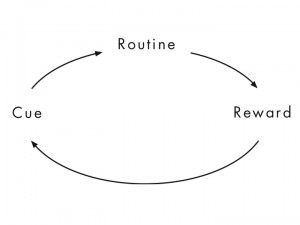
\includegraphics[width=0.4\textwidth]{images/habitloopbasic.jpg}
\caption{The basic habit loop}
\end{figure}
\newline The next issue many encounter is that identifying all the elements of a habit is tricky. For example, a cue related to a habit can consist of many pieces of information, perhaps a time, a place, an emotion, or even a person, the list is endless. This makes it very difficult for people to pinpoint what their exact habit loop looks like. Though people may estimate, accuracy is imperative here. This made the focus of our application more clear; instead of simply allowing users to track their habits and habit loops, our application actually help users discover their unique detailed habit loop.
\newline \newline
We studied the methodology Duhigh lays out in the book, and decided that integrating it into a piece of software would be perfect in creating a habit tracker that 1) employs the concepts of the habit loop, and 2) is educational and allows people to discover their actual habit loops, as opposed to having them blindly enter what they \textit{believe} is their habit loop.

\subsection{Building a Habit}
\subsubsection*{Step One: Identify the Routine}
The first step in diagnosing a habit is determining what the exact habit is. In particular, the action that is repeatedly being performed is defined as the routine. For example, one may immediately open the Instagram app on their phone in bed when they wake up. Thus, the routine here is opening Instagram on their phone. A common approach taken by many in efforts to break this habit is trying to ignore the habit by getting out of bed immediately. This may be effective for a couple of days before going back to their old ways. Though seemingly harmless at first, thoughts such as ”I have lots of time to get to work”, and ”what is another 5 minutes” may feel good for a while, but eventually will turn sour. Ultimately, a cyclical ”I will do it tomorrow” attitude is created.
\newline \newline
Needless to say, identifying the routine is the first step towards creating a habit loop. The routine is often rather obvious, however the following steps can be quite the opposite.
\subsubsection*{Step Two: Experiment with Rewards}
After identifying the routine, the user needs to determine what is so compelling about the routine, more precisely, what is the reward. These rewards can be extremely powerful as they often satisfy cravings. These cravings are quite often an unconscious desire, in the case of social media, there have been countless studies on how the brain develops an addiction. The result is that the person is then driven by an uncontrollable urge to log onto or use social media. At the end of the day, the reward is an occurrence that triggers one’s brain to release dopamine.
\newline \newline
Now, the key here is to experiment with alternative routines that trigger the same reward. Perhaps in the case of wanting to open Instagram, an alternative routine could be reading 5 pages of a book, or getting up and doing jumping jacks. The main objective is that whatever the activity is, it must be able to satisfy the craving, and finding something that is able to fulfill this, often takes experimentation. Perhaps the first day you try activity A, then B on the next, then C, and so on. The point is to test various hypotheses in efforts to determine what desire is actually driving the routine. Moreover, does the user crave going on Instagram, or are they just trying to procrastinate going to work? Unfortunately, Instagram is favorable as it happens to be a convenient distraction that does not require leaving your bed.
\subsubsection*{Step Three: Isolate the Cue}
The third step is then to identify the cue, which can be difficult for many. ”When you automatically turn your car left while driving to work, what triggers that behavior? A street sign? A particular tree? The knowledge that this is, in fact, the correct route? All of them together?”\footnote{\url{https://charlesduhigg.com/how-habits-work/}}. In the case of the aforementioned example, is the person going on Instagram because they think they want to look for something in particular, or is it just what they have become accustomed to do. The cue can be a very complicated to construct, and can consist of many things. Here are some examples of common cue categories:
\begin{itemize}
    \item Location
    \item Time
    \item Mood
    \item Thoughts
    \item Surrounding people
    \item A certain song
\end{itemize}
\subsubsection*{Step Four: Have a Plan}
At this point the person has determined their habit loop. That which includes the reward, the cue, and the routine, from here they are able to shift their behaviour toward a successful alternative routine. To put it differently, a habit is a formula the human brain automatically follows: ”When I see a \textbf{cue}, I will do a \textbf{routine} in order to get a \textbf{reward}”. Essentially, the goal is to engrave this new formula. Now, the question for us as the engineers is how can we build a software engineering solution that enables people to follow these steps and achieve greater success had they not used our development.
